\chapter{DESKRIPSI SUB SISTEM}

Karena sistem yang akan dibuat menggunakan desain berorientasi objek, maka penjelasan lebih detail dari sub-sistem ini akan lebih mudah bila kita melihat diagram \textit{class} yang telah dijelaskan dan digambarkan pada bagian sebelumnya, namun kali ini akan dijelaskan lebih detail.

\section{Kelas AppInitializer}

Kelas ini menjadi kelas pembuka bagi sistem aplikasi yang menggunakan \textit{framework} Spring karena kelas ini mengimplementasikan \textit{interface} dari \textit{framework} Spring yang bernama AbstractAnnotationConfigDispatcherServletInitializer.

Diagram dari kelas AppInitializer ini seperti ditunjukkan pada gambar \ref{fig:uml-class-AppInitializer} :

\begin{figure}[H]
  \centering
  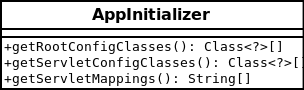
\includegraphics[width=0.5\textwidth]{./resources/uml/uml-class-AppInitializer}
  \caption{Diagram Kelas AppInitializer}
  \label{fig:uml-class-AppInitializer}
\end{figure}

Karena kelas ini adalah implementasi dari \textit{interface} AbstractAnnotationConfigDispatcherServletInitializer, maka harus mengimplementasikan pula ketiga \textit{method} yang ada pada \textit{interface} tersebut, yaitu \textit{method} getRootConfigClasses, \textit{method} getServletConfigClasses, dan \textit{method} getServletMappings.

\section{Kelas AppConfig}

Kelas ini merupakan kelas konfigurasi yang digunakan \textit{framework} Spring untuk melakukan konfigurasi terhadap sistem aplikasi yang akan dijalankan. Bukan karena mengimplementasikan kelas atau \textit{interface} yang dibawa oleh Spring, melainkan karena dideklarasikan sebagai kelas yang menangani konfigurasi sistem aplikasi di kelas AppInitializer.

Pada kelas ini, karena menggunakan fitur MVC (\textit{Model-View-Controller}) dari Spring, maka akan ada beberapa kelas yang ditujukan untuk fungsinya masing-masing, dikelas inilah nantinya kelas-kelas tersebut dideklarasikan, pada kelas ini pula disebutkan kelas yang bertanggung jawab untuk melakukan konfigurasi-konfigurasi yang lain termasuk konfigurasi komunikasi dengan sistem basis data.

Diagram dari kelas AppConfig ini seperti ditampilkan pada gambar \ref{fig:uml-class-AppConfig} :

\begin{figure}[H]
  \centering
  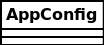
\includegraphics[width=0.3\textwidth]{./resources/uml/uml-class-AppConfig}
  \caption{Diagram Kelas AppConfig}
  \label{fig:uml-class-AppConfig}
\end{figure}

Kelas ini memang terlihat kosong, karena konfigurasi-konfigurasi yang dilakukan nantinya akan menggunakan fitur \textit{annotation} milik Java agar memudahkan pembacaan kode dan menyederhanakan konfigurasi.

\section{Kelas HibernateConfiguration}

Kelas ini bertugas melakukan konfigurasi komunikasi dengan sistem basis data. Diagram dari kelas HibernateConfiguration ini seperti terlihat pada gambar \ref{fig:uml-class-HibernateConfiguration} :

\begin{figure}[H]
  \centering
  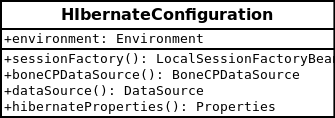
\includegraphics[width=0.8\textwidth]{./resources/uml/uml-class-HibernateConfiguration}
  \caption{Diagram Kelas HibernateConfiguration}
  \label{fig:uml-class-HibernateConfiguration}
\end{figure}

Kelas ini terdiri dari 1 (satu) properti dan 4 (empat) \textit{method}. Propertinya diberi nama environment, karena properti ini akan bertugas menampung nilai-nilai konfigurasi standar yang berada pada \textit{file} yang terpisah.

\textit{Method} yang pertama adalah \textit{method} sessionFactory. \textit{Method} sessionFactory ini akan bertugas mengembalikan nilai sebuah kelas LocalSessionFactoryBean dimana kelas ini yang menjadi sesi dari tiap \textit{user} untuk melakukan koneksi ke basis data nantinya. Untuk menyediakan akses data yang cepat dan optimal, \textit{method} ini akan menggunakan \textit{connection pool} milik BoneCP.

\textit{Method} berikutnya adalah boneCPDataSource, \textit{method} ini akan menyediakan konfigurasi untuk melakukan koneksi ke basis data sebagai sumber data, yang dikembalikan dalam bentuk kelas BoneCPDataSource. \textit{Method} ini menjadi sumber untuk pengambilan data apapun pada basis data dengan menggunakan \textit{connection pool} BoneCP.

\textit{Method} dataSource adalah \textit{method} standar yang menggunakan \textit{connection pool} yang dibawa oleh Hibernate yang digunakan untuk melakukan pemeriksaan awal koneksi ke basis data, apabila menggunakan \textit{method} ini berhasil, maka tidak akan menjadi masalah apabila dilakukan menggunakan \textit{connection pool} yang lain.

\textit{Method} yang terakhir adalah hibernateProperties, \textit{method} ini melakukan konfigurasi terhadap Hibernate yang nantinya digunakan pada \textit{method} sessionFactory.

\section{Kelas SpptRestController}

Kelas ini yang menjadi gerbang pertama yang menentukan kemana sebuah \textit{request} akan di respon. Diagram kelas dari SpptRestController ini akan terlihat seperti pada gambar \ref{fig:uml-class-SpptRestController} :

\begin{figure}[H]
  \centering
  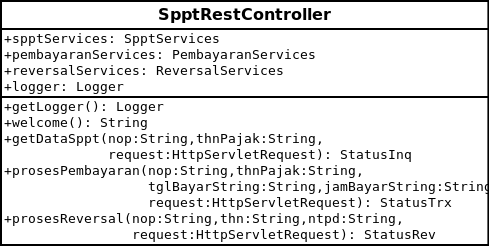
\includegraphics[width=0.8\textwidth]{./resources/uml/uml-class-SpptRestController}
  \caption{Diagram Kelas SpptRestController}
  \label{fig:uml-class-SpptRestController}
\end{figure}

Kelas ini memiliki 4 (empat) properti dan 5 (lima) \textit{method}. Penjelasan dan fungsi masing-masing properti dan \textit{method} tersebut yaitu sebagai berikut :

\begin{itemize}
  \item Properti
  
  \begin{itemize}
    \item Properti spptServices
    
    Properti ini yang akan mengatur layanan yang menangani permintaan / \textit{request inquiry} dari \textit{client}.
    
    \item Properti pembayaranServices
    
    Properti pembayaranServices ini akan mengatur layanan yang menangani permintaan / \textit{request} pencatatan pembayaran dari \textit{client}.
    
    \item Properti reversalServices
    
    Properti reversalServices ini akan mengatur layanan yang menangani permintaan / \textit{request reversal} dari \textit{client} karena ada kesalahan pencatatan pembayaran sebelumnya.
    
    \item Properti logger
    
    Properti logger digunakan untuk melakukan pencatatan aktifitas sistem aplikasi ke dalam sebuah \textit{file} pada saat sistem aplikasi berjalan dan digunakan. Kondisi ini diperlukan agar memudahkan diagnosa sistem apabila terjadi anomali-anomali proses yang tidak diinginkan.
   
  \end{itemize}
  
  \item \textit{Method}
  
  \begin{itemize}
    \item \textit{Method} getLogger
    
    \textit{Method} getLogger ini menyediakan akses ke properti logger agar dapat mencatat kejadian saat \textit{runtime} dari kelas mana pun pada sistem aplikasi.
    
    \item \textit{Method} welcome
    
    \textit{Method} welcome ini adalah halaman muka dari layanan Rest, jadi setiap \textit{request} yang dilayangkan ke \textit{root slash} ("/"), maka akan direspon oleh \textit{method} welcome ini.
    
    \item \textit{Method} getDataSppt
    
    \textit{Method} getDataSppt difungsikan sebagai tempat masuknya \textit{request inquiry} data tagihan SPPT PBB-P2, nantinya \textit{method} ini akan mengembalikan respon dalam bentuk kelas StatusInq yang telah diubah dalam format JSON.
    
    \item \textit{Method} prosesPembayaran
    
    \textit{Method} prosesPembayaran ini akan bertugas menangani \textit{request} pencatatan pembayaran dari \textit{client}. \textit{Method} ini akan mengembalikan kelas StatusTrx yang tentunya telah diubah dalam format JSON.
    
    \item \textit{Method} prosesReversal
    
    \textit{Method} prosesReversal ini seperti \textit{method} getDataSppt dan \textit{method} prosesPembayaran yang menangani sebuah \textit{request} dari \textit{client}, namun \textit{method} prosesReversal ini akan menangani \textit{request reversal} dari pembayaran yang telah tercatat dalam basis data.
    
    Penyebab proses \textit{reversal} ini karena adanya kesalahan pencatatan pembayaran yang sebelumnya terjadi, misalkan pada saat \textit{client} melakukan \textit{request} pencatatan pembayaran, sebelum \textit{client} mendapatkan respon dari \textit{server} koneksi tiba-tiba terputus dan \textit{client} tidak pernah mendapatkan respon atas \textit{request}-nya, maka untuk memastikan adalah melakukan \textit{request reversal} dan melakukan \textit{request} pencatatan pembayaran kembali.
    
  \end{itemize}
\end{itemize}

\section{Kelas SpptServicesImpl}

Kelas SpptServicesImpl akan melayani \textit{request inquiry} dan melanjutkannya ke kelas-kelas yang menangani basis data. Diagram kelas dari SpptServicesImpl ini adalah seperti pada gambar \ref{fig:uml-class-SpptServicesImpl}

\begin{figure}[H]
  \centering
  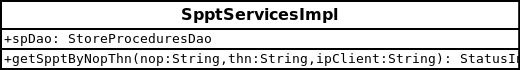
\includegraphics[width=1\textwidth]{./resources/uml/uml-class-SpptServicesImpl}
  \caption{Diagram Kelas SpptServicesImpl}
  \label{fig:uml-class-SpptServicesImpl}
\end{figure}

Kelas SpptServicesImpl ini memiliki 1 (satu) properti dan 1 (satu) \textit{method}. Propertinya bernama spDao, untuk menampung kelas StoreProceduresDao yang menangani semua hal mengenai eksekusi \textit{store procedure} pada basis data.

\textit{Method} dari kelas ini bernama getSpptByNopThn yang berfungsi melakukan pemanggilan terhadap kelas yang bertugas menghubungi basis data yang pencarian datanya berdasarkan Nomor Objek Pajak (NOP) dan tahun pajak.

\section{Kelas PembayaranServicesImpl}

Kelas PembayaranServicesImpl bertugas melayani permintaan terhadap pencatatan pembayaran yang posisinya berada di tengah dan menjadi penghubung antara \textit{interface} dengan kelas-kelas \textit{data access}. Diagram kelas PembayaranServicesImpl ini seperti pada gambar \ref{fig:uml-class-PembayaranServicesImpl} :

\begin{figure}[H]
  \centering
  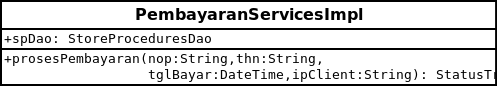
\includegraphics[width=1\textwidth]{./resources/uml/uml-class-PembayaranServicesImpl}
  \caption{Diagram Kelas PembayaranServicesImpl}
  \label{fig:uml-class-PembayaranServicesImpl}
\end{figure}

Kelas ini memiliki 1 (satu) properti dan 1 (satu) \textit{method}, properti yang dimiliki bernama spDao, ini adalah instan dari kelas atau \textit{interface} StoreProceduresDao yang bertugas melakukan komunikasi dengan sistem aplikasi basis data.

Sedangkan \textit{method} prosesPembayaran adalah \textit{method} yang bertugas sebagai penghubung antara \textit{interface} dalam hal ini kelas SpptRestController, dengan kelas yang berhubungan dan berkomunikasi langsung dengan basis data untuk melakukan eksekusi pencatatan pembayaran.

\section{Kelas ReversalServicesImpl}

Seperti kelas PembayaranServicesImpl dan SpptServicesImpl, kelas ReversalServicesImpl bertugas menjadi penghubung antara \textit{interface} yang menangani 

\section{Kelas StoreProceduresDaoImpl}

\section{Kelas StatusInq}

\section{Kelas StatusTrx}

\section{Kelas StatusRev}

\section{Kelas Sppt}

\section{Kelas PembayaranSppt}

\section{Kelas ReversalPembayaran}